\documentclass{beamer}
\usepackage[utf8]{inputenc}
\usepackage{amsmath}
\usepackage{graphicx}
\usepackage{parskip}
\setlength{\parskip}{\smallskipamount}
\usepackage{fontenc}
\graphicspath{{./images/}}
\usetheme{PaloAlto}
\usecolortheme{wolverine}
\renewcommand{\baselinestretch}{1.3}
\setbeamercolor{block title}{bg=black}

\title{Matrix Project}
\author[]{K.Surya Prakash EE18BTECH11026\\
          D.Krishna Srikar EE18BTECH11014}


\begin{document}

\maketitle

\begin{frame}{Question:}

\begin{block}{In Geometry}
Q.Find the shortest distance between the line $y = x+1$ and the parabola $y^2 = x$(JEE-MAIN 2009).
\end{block}
\\
\begin{block}{In Matrices}
Q. Find the shortest distance between the line   
$
\begin{bmatrix}
1&-1\\
\end{bmatrix}x + 1= 0$ and the parabola 
$x^T \begin{bmatrix}
0&0\\
0&1\\
\end{bmatrix}$x -
$\begin{bmatrix}
1&0\\
\end{bmatrix}x  = 0$
\end{block}
\\
Ans: \(\frac{3\sqrt{2}}{8}\)  = 0.53

\end{frame}


\begin{frame}{Graphical Representation:}
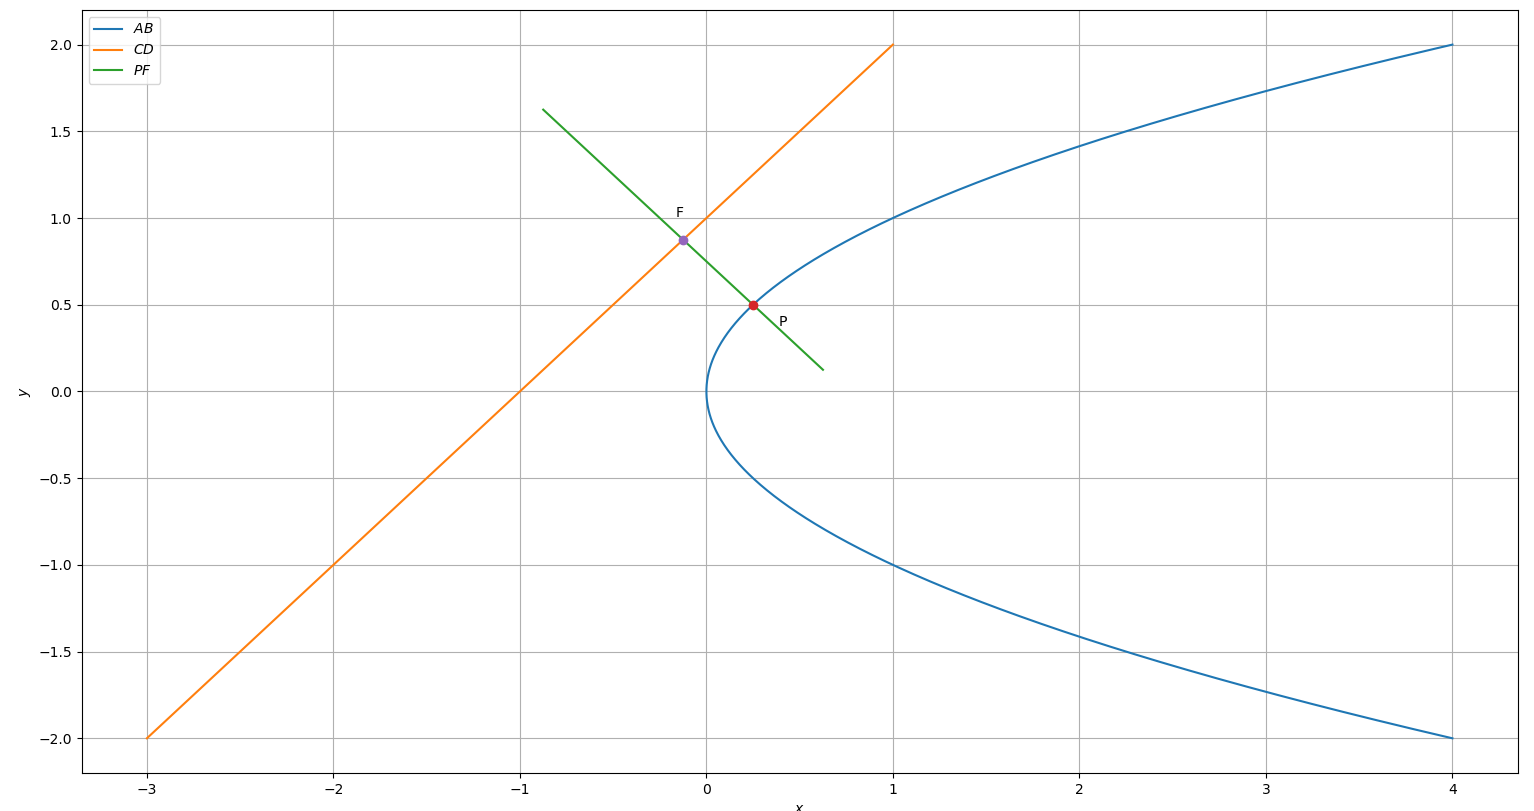
\includegraphics[scale = 0.185]{plot}
\end{frame}

\begin{frame}{Solution:}

Sol) Let 'n' be the direction vector matrix  of the given line $x - y + 1 = 0$

$$
n = \begin{bmatrix}
-1 \\
1\\
\end{bmatrix}
$$

Let P is a point on the parabola having tangent parallel to given line then the perpendicular drawn from P to the give line has the shortest distance.

$$P =
\begin{bmatrix}
a\\
b
\end{bmatrix}$$

\end{frame}


\begin{frame}{Equation of Parabola}
General equation of a conic is $x^TVx + 2u^Tx + F = 0$. Given equation of parabola
$x^T \begin{bmatrix}
0&0\\
0&1\\
\end{bmatrix}$x -
$\begin{bmatrix}
1&0\\
\end{bmatrix}x  = 0$\\
On comparing the two equations 
V = \begin{bmatrix}
0&0\\
0&1\\
\end{bmatrix} ,
u = \begin{bmatrix}
-0.5&0
\end{bmatrix} and F = 0.\\

\end{frame}


\begin{frame}{Equations of Tangents}
\textbullet The equation of Tangent at P to the parabola is given as:
\begin{center}
$X^Tn+c = 0$
\end{center}
which can also be written as
\begin{center}
$n^TX+c = 0$ (Since $n^TX = X^Tn$)\\
\end{center}
General equation of tangent at P to the conic is $(P^TV+u^T)+P^Tx + F = 0$ and by substituting the values of P,V,F and u we will get the equation of tangent as
$$
\begin{bmatrix}
0.5&b
\end{bmatrix}
%
\begin{bmatrix}
x\\
y\\
\end{bmatrix} +  \frac{-a}{2}\ = 0
$$ 

\end{frame}


\begin{frame}{Calculating the Co-ordinates of point P}{\textwidth}
On comparing the equations of tangents we will get 
n^T = k(\begin{bmatrix}
-0.5&0
\end{bmatrix}).
\\We know that 
n = \begin{bmatrix}
-1\\
1\\
\end{bmatrix} so $(-0.5)k = 1$
\Rightarrow k = 2\\
\Rightarrow b = 0.5\\
\Rightarrow a = 0.25 (\text{As P lie on parabola $y^2 = x$})\\
\Rightarrow
P = \begin{bmatrix}
0.25\\
0.5\\
\end{bmatrix}
    
\end{frame}

\begin{frame}{Formula for shortest distance:}
\starShortest Shortest distance(d) from a point to line is the perpendicular distance drawn from the point to the line, which is given by
\begin{center}

$d = \frac{|P^Tn + 1|}{||n||}$;
 where $||n|| = \sqrt{n[0]^2 + n[1]^2}\\$
d = \(\frac{3\sqrt{2}}{8}\)
\end{center}
\end{frame}


\begin{frame}{Graphical Representation:}
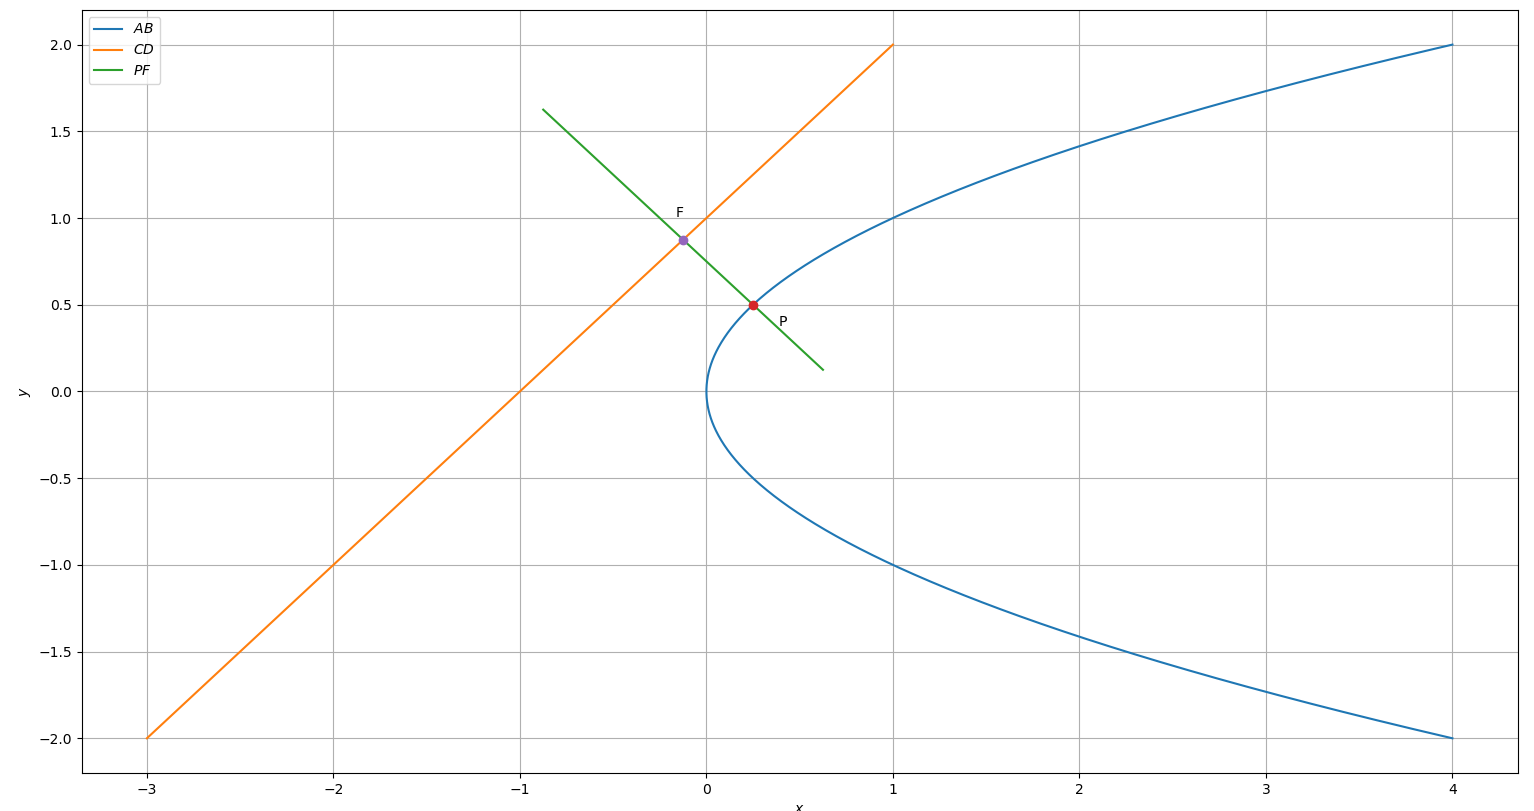
\includegraphics[scale = 0.185]{plot}\\
So, the shortest distance between parabola and line $x - y + 1 = 0$ is equal to $\frac{3\sqrt{2}}{8}\ $ units.
\end{frame}

\end{document}
